\documentclass[]{elsarticle} %review=doublespace preprint=single 5p=2 column
%%% Begin My package additions %%%%%%%%%%%%%%%%%%%
\usepackage[hyphens]{url}

  \journal{Lancet: Global Health} % Sets Journal name


\usepackage{lineno} % add
  \linenumbers % turns line numbering on
\providecommand{\tightlist}{%
  \setlength{\itemsep}{0pt}\setlength{\parskip}{0pt}}

\usepackage{graphicx}
\usepackage{booktabs} % book-quality tables
%%%%%%%%%%%%%%%% end my additions to header

\usepackage[T1]{fontenc}
\usepackage{lmodern}
\usepackage{amssymb,amsmath}
\usepackage{ifxetex,ifluatex}
\usepackage{fixltx2e} % provides \textsubscript
% use upquote if available, for straight quotes in verbatim environments
\IfFileExists{upquote.sty}{\usepackage{upquote}}{}
\ifnum 0\ifxetex 1\fi\ifluatex 1\fi=0 % if pdftex
  \usepackage[utf8]{inputenc}
\else % if luatex or xelatex
  \usepackage{fontspec}
  \ifxetex
    \usepackage{xltxtra,xunicode}
  \fi
  \defaultfontfeatures{Mapping=tex-text,Scale=MatchLowercase}
  \newcommand{\euro}{€}
\fi
% use microtype if available
\IfFileExists{microtype.sty}{\usepackage{microtype}}{}
\bibliographystyle{elsarticle-harv}
\usepackage{longtable}
\usepackage{graphicx}
\ifxetex
  \usepackage[setpagesize=false, % page size defined by xetex
              unicode=false, % unicode breaks when used with xetex
              xetex]{hyperref}
\else
  \usepackage[unicode=true]{hyperref}
\fi
\hypersetup{breaklinks=true,
            bookmarks=true,
            pdfauthor={},
            pdftitle={Combining Rapid Antigen Testing and Syndromic Data Improves Sensitivity and Specificity in Real-World COVID-19 Detection},
            colorlinks=false,
            urlcolor=blue,
            linkcolor=magenta,
            pdfborder={0 0 0}}
\urlstyle{same}  % don't use monospace font for urls

\setcounter{secnumdepth}{5}
% Pandoc toggle for numbering sections (defaults to be off)

% Pandoc citation processing
\newlength{\cslhangindent}
\setlength{\cslhangindent}{1.5em}
\newlength{\csllabelwidth}
\setlength{\csllabelwidth}{3em}
% for Pandoc 2.8 to 2.10.1
\newenvironment{cslreferences}%
  {}%
  {\par}
% For Pandoc 2.11+
\newenvironment{CSLReferences}[2] % #1 hanging-ident, #2 entry spacing
 {% don't indent paragraphs
  \setlength{\parindent}{0pt}
  % turn on hanging indent if param 1 is 1
  \ifodd #1 \everypar{\setlength{\hangindent}{\cslhangindent}}\ignorespaces\fi
  % set entry spacing
  \ifnum #2 > 0
  \setlength{\parskip}{#2\baselineskip}
  \fi
 }%
 {}
\usepackage{calc}
\newcommand{\CSLBlock}[1]{#1\hfill\break}
\newcommand{\CSLLeftMargin}[1]{\parbox[t]{\csllabelwidth}{#1}}
\newcommand{\CSLRightInline}[1]{\parbox[t]{\linewidth - \csllabelwidth}{#1}\break}
\newcommand{\CSLIndent}[1]{\hspace{\cslhangindent}#1}

% Pandoc header
\renewenvironment{abstract}{}{}
\usepackage[colorinlistoftodos]{todonotes}
\usepackage{booktabs}
\usepackage{longtable}
\usepackage{array}
\usepackage{multirow}
\usepackage{wrapfig}
\usepackage{float}
\usepackage{colortbl}
\usepackage{pdflscape}
\usepackage{tabu}
\usepackage{threeparttable}
\usepackage{threeparttablex}
\usepackage[normalem]{ulem}
\usepackage{makecell}
\usepackage{xcolor}



\begin{document}
\begin{frontmatter}

  \title{Combining Rapid Antigen Testing and Syndromic Data Improves Sensitivity and Specificity in Real-World COVID-19 Detection}
    \author[IBAHCM,UoGLMICS]{Fergus J Chadwick}
   \ead{f.chadwick.1@research.gla.ac.uk} 
    \author[IBAHCM,UoGLMICS]{Yacob Haddou}
   \ead{yacob.haddou@glasgow.ac.uk} 
    \author[IBAHCM]{Tasnuva Chowdhury}
   \ead{tasnuvachowdhury2004@gmail.com} 
    \author[MRCB]{David Pascall}
   \ead{david.pascall@mrc-bsu.cam.ac.uk} 
    \author[a2i]{Shayan Chowdhury}
   \ead{shayan.chowdhury@a2i.gov.bd} 
    \author[IBAHCM,UoGLMICS]{Jessica Clark}
   \ead{Jessica.Clark@glasgow.ac.uk} 
    \author[UNFAO]{Joanna Andrecka}
   \ead{aandrecka@gmail.com} 
    \author[MathsandStatGla,UoGLMICS]{Mikolaj Kundergorski}
   \ead{mikolaj.kundegorski@gmail.com} 
    \author[MathsandStatGla,UoGLMICS]{Craig Wilkie}
   \ead{craig.wilkie@glasgow.ac.uk} 
    \author[UNFAO]{Eric Brum}
   \ead{eric.brum@fao.org} 
    \author[IEDCR]{Tahmina Shirin}
   \ead{tahmina.shirin14@gmail.com} 
    \author[IEDCR]{A S M Alamgir}
   \ead{aalamgir@gmail.com} 
    \author[IEDCR]{Mahbubur Rahman}
   \ead{dr\_mahbub@yahoo.com} 
    \author[IEDCR]{Ahmed Nawsher Alam}
   \ead{anawsher@yahoo.com} 
    \author[IEDCR]{Farzana Khan}
   \ead{farzanakhan\_25@yahoo.com} 
    \author[MathsandStatGla,UoGLMICS]{Janine Illian}
   \ead{janine.illian@glasgow.ac.uk} 
    \author[MathsandStatGla,UoGLMICS]{Ben Swallow}
   \ead{ben.swallow@glasgow.ac.uk} 
    \author[IBAHCM,UoGLMICS]{Davina L Hill}
   \ead{davina.hill@glasgow.ac.uk} 
    \author[MathsandStatGla]{Dirk Husmeier}
   \ead{dirk.husmeier@glasgow.ac.uk} 
    \author[IBAHCM,UoGLMICS]{Jason Matthiopoulos}
   \ead{jason.matthiopoulos@glasgow.ac.uk} 
    \author[IBAHCM,UoGLMICS]{Katie Hampson}
   \ead{katie.hampson@glasgow.ac.uk} 
    \author[Columbia]{Ayesha Sania}
   \ead{ays328@mail.harvard.edu} 
      \address[IBAHCM]{Institute of Biodiversity, Animal Health and Comparative Medicine, University of Glasgow}
    \address[UoGLMICS]{COVID-19 in LMICs Research Group, University of Glasgow}
    \address[MRCB]{MRC Biostatistics Unit, University of Cambridge}
    \address[MathsandStatGla]{School of Mathematics and Statistics, University of Glasgow}
    \address[a2i]{a2i Programme, ICT Ministry/UNDP Bangladesh}
    \address[UNFAO]{UN FAO in support of the UN Interagency Support Team, Bangladesh}
    \address[IEDCR]{Institute of Epidemiology, Disease Control and Research, Ministry of Health, Bangladesh}
    \address[Columbia]{Division of Developmental Neuroscience, Department of Psychiatry, Columbia University}
      \cortext[1]{Corresponding Author}
  
  \begin{abstract}
  
  \end{abstract}
  
 \end{frontmatter}

\hypertarget{abstract-max-250-words---currently-over}{%
\section{Abstract (Max 250 Words - Currently over)}\label{abstract-max-250-words---currently-over}}

\emph{Background}

The majority of the world's population live in low- and middle-income countries (LMICs) where access to gold-standard diagnostics like RT-PCR is often limited.
Rapid antigen testing (RAT) and syndromic diagnosis are two alternative, inexpensive and easy-to-deploy surveillance methods but there are concerns that they lack the sensitivity and specificity to effectively guide practice.

\emph{Methods}

Bangladesh's Institute of Epidemiology Disease Control And Research (IEDCR) identified potential COVID-19 patients in Dhaka using syndromic surveillance.
A sample (n = 1172) of these patients was tested using RAT and syndromic data were collected.
Models were fit to predict RT-PCR status using the RAT data, the syndromic data, and the two combined.
Model performance was measured using predictive power and classification performance under three epidemiological scenarios: ``Agnostic,'' ``Rising Cases'' and ``Low-Level Cases.''

\emph{Findings}

Combined data models yielded equal or improved performance over syndromic- and RAT-only models across all three epidemiological scenarios and when compared as more generic prediction and classification engines.
In the ``Rising Cases'' scenario, which most closely represents the current situation in many LMICs, the combined data model false negative rate is 26 percentage points lower that of the RAT only model.
Although the syndromic only model matches the combined models false negative rate, its false positive rate is 31 percentage points higher.

\emph{Interpretation}

A few accurate tests may be less useful at the population level than many more imperfect ones.
Small, scalable improvements in the accuracy of mass-deployed but imperfect tests can then make a very big difference for pandemic control.\\
We demonstrate that such improvements can be achieved by statistically utilising complementary strengths and weaknesses across two imperfect diagnostics, we can greatly improve the detection of COVID-19.

\emph{Funding}

The Bill and Melinda Gates Foundation and the Wellcome Trust.

\hypertarget{introduction-1107-words}{%
\section{Introduction (\textasciitilde1107 Words)}\label{introduction-1107-words}}

Identification and isolation of COVID-19 cases remains key to the pandemic response across the globe.
The faster and more accurately we can identify cases, the more effectively we can provide clinical care, reduce transmission of infection and develop population-level interventions.
RT-PCR testing has rapidly become the default, gold-standard test for COVID-19 in applied settings due to its high sensitivity and specificity for COVID-19 {[}2{]}.
Most of the world's population, however, live in low- and middle-income countries (LMICs) where the laboratory facilities needed to carry out RT-PCR tests are often scarce and hard to reach {[}4{]}.
COVID-19 diagnosis worldwide, therefore, must be made accessible using inexpensive methods that can be carried out locally {[}6{]}.

An increasingly popular alternative to RT-PCR is rapid antigen testing (RAT) {[}7{]}.
Like RT-PCR, these tests have high specificity for COVID-19 while being less expensive, easier to implement, and faster to produce results {[}8{]}.
RATs also require less commitment and discomfort for patients.
For RT-PCR testing, patients must travel to a designated site (such as a hospital or testing booth) or have highly visible PPE-clad officials visit their home.
Then, invasive nasopharyngeal swabs must be taken and there is a delay in receiving the result (between one day and a week in Bangladesh).
In contrast, RAT can be conducted on nasal or saliva samples, completed in the home with minimal PPE and results are available in 30 minutes.
RATs can be taken by persons with limited training, thus decreasing the time and expense associated with identifying cases.
Together, these traits make RATs an appealing alternative to RT-PCR.
However, several concerns have been raised about the sensitivity of RAT {[}9{]} leading to more false negative diagnoses.

Another alternative to RT-PCR, one that has been used since the start of the pandemic, is identifying cases through symptom-thresholding\todo{Not an official term} {[}10{]}.
In this approach, a patient presenting with a fever and one or more viral pneumonia symptoms is treated as a COVID-19 positive patient.
The main advantage of this approach is the ease of implementation.
As with RAT the process is faster, cheaper and less invasive than RT-PCR, but unlike RAT the process relies on minimal equipment and thus can be scaled quickly and easily.
For example, in Bangladesh, an LMIC, much of the initial support and reporting of infections locally is provided by community support teams (CSTs) composed of local volunteers with basic training.
The CSTs can easily collect symptomatic data in the community and provide care where the thresholds are met.
However, these thresholds were developed early in the outbreak, and thus were necessarily drawn from clinical intuition, rather than data, and for different variants and populations than they are now applied to.
Consequently, the relationship between the thresholds and the true COVID-19 status is often weak, with low specificity leading to a very large number of false positive diagnoses.

A natural extension to these symptom-threshold approaches is syndromic modelling.
Here, a patient presenting with a fever and one or more viral pneumonia symptoms is treated as a potential COVID-19 patient.
However, rather than using a set of pre-determined criteria, a range of symptomatic and risk factor data are collected and then a sub-sample of patients is tested using RT-PCR for COVID-19 {[}11{]}.
These data are used to fit a model that allows more accurate prediction of how likely a patient is to have COVID-19 through the identification of COVID-19 syndromes {[}13{]}.
It is worth highlighting at this point that in resource-limited settings, there is very limited provision for testing of asymptomatic cases, despite their important role in disease transmission {[}14{]}.
Even while focusing solely on symptomatic patients, syndromic modelling is a complex and nuanced task.
The strength of relationships between symptoms and diseases is not stable through time or across sampling strategies since the relative importance of each symptom for disease diagnosis, in part, depends on the prevalence of other diseases causing similar symptoms in the community {[}15{]}.
For example, if another disease for which loss of smell is a symptom becomes common, that symptom becomes a worse predictor for COVID-19.
Similarly, if everyone who presents has a cough and thus is included in the sample, then coughing will likely have a very low correlation with COVID-19 (even if the two are strongly related in the general population).
Symptoms are also inter-related, meaning that they cannot be interpreted independently.
The majority of methods used currently do not account for these changes through time, symptom-to-symptom correlations or the relationship between the population sampled and the target population.
Even then, the many types of common respiratory disease generally means that even then these models tend to have relatively high false positive rates (low specificity) for COVID-19 {[}15{]}, although much lower than the symptom-threshold approach.

Poor sensitivity and specificity are problematic in diagnostics but higher error rates than gold-standard methods may be tolerable depending on their scale and impact given the local situation.
Low specificity means a large number of false positive classifications, where the patient is told they have COVID-19 but they actually do not.
This might lead to patients unnecessarily self-isolating and receiving support which can be expensive to the individuals and local public health bodies, as well as reducing available resources for those who need them {[}16{]}.
Similarly, low sensitivity means more false negative classifications, where the patient is told they do not have COVID-19 but they actually do, which can lead to a health-risk for the individual and to the disease spreading further {[}17{]}.
The costs of these misclassifications will depend on local context.
When the prevalence of the disease is low, false positives may create local scepticism about the value of testing, or when there are strong population-level mitigations already in place (such as a nationwide lockdown), then false positives might be more costly than false negatives {[}16{]}.
If the disease is abundant or increasing rapidly then false negatives are likely to be more costly.
In most situations, a balance will need to be struck {[}4{]}.

The two dominant ``alternative'' testing methods available in resource limited settings, therefore, are both flawed.
Relying solely on symptomatic diagnosis will likely overestimate the number of individuals with COVID-19 due to its lack of specificity.
Conversely, RATs will give a false impression of control due to the number of positive cases that will be missed.
In this paper, we demonstrate how to combine these data types to exploit their complementarity and amelioriate their respective weaknesses.
We aim to compare the performance of these two testing methods and the combined approach both in terms of general prediction and as diagnostics under three epidemiological scenarios; and demonstrate that the combined data achieve equal to much lower error rates than the next best method.
We then discuss the role of statistically integrating data from multiple imperfect testing methods in resource limited settings to improve the diagnosis of diseases, particularly COVID-19.

\hypertarget{methods-1019-words}{%
\section{Methods (\textasciitilde1019 Words)}\label{methods-1019-words}}

Participants included in this study were identified for COVID-19 testing after self-reporting symptoms to the Bangladesh government's national hotlines for COVID-19 support.
Recruitment took place across Dhaka (the capital city of Bangladesh) between 2nd April 2021 and 5th May 2021.

Patients were selected for further testing conditional on the presence of a fever (\textgreater38°C) at the point of testing and one or more of 14 additional symptoms associated with COVID-19 (breathing problems, coughing, diarrhoea, fever (ongoing), a headache, loss of taste, loss of smell, muscle pain, red eyes, a runny nose, a sore throat, tiredness, vomiting or a wet cough).
The patient's age and gender were also recorded, but these data were not included in the patient selection criteria.

Nasal swabs and syndromic data were collected from the patient by medical technologists.
One swab each was used for rapid antigen testing (RAT) and RT-PCR (gold-standard for COVID-19 status).
The full questionnaire and testing protocols are provided in Appendix XX.
Participants provided written informed consent to sample collection and for their test results to be analyzed in the study.

\begin{figure}
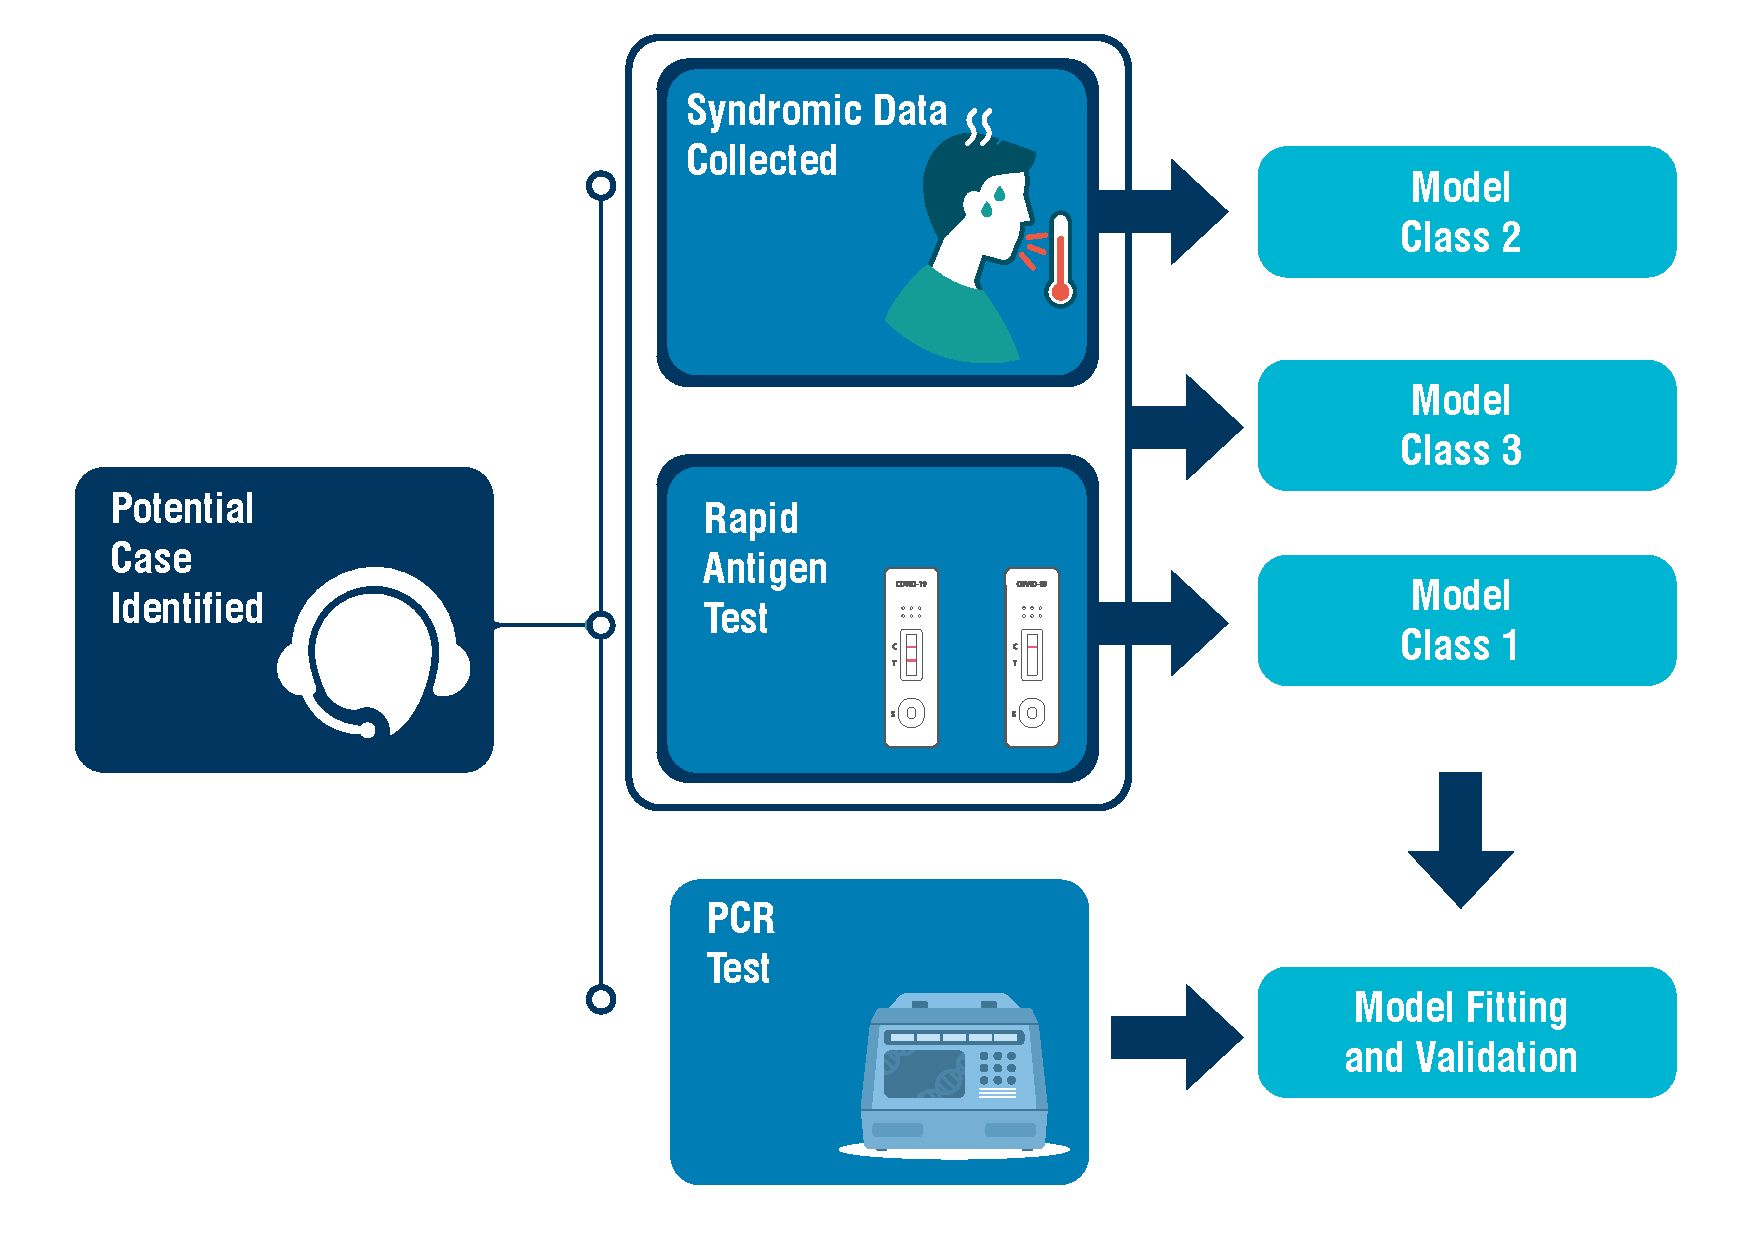
\includegraphics[width=1\linewidth]{/home/fergus/Git/COVID19_SyndromicRATDiagnosis/0500_Manuscript/0501_MainText/MainTextFigs/DataFlowchart} \caption{Schematic description of identification of likely COVID-19 patients by community support teams (CSTs), swab collection and model definitions. The teams collected syndromic data (age, gender and presence/absence of 14 predetermined symptoms), and two sets of naso-pharyngeal swabs (one each for Rapid Antigen Testing and RT-PCR). We then used rapid antigen testing (RAT) and syndromic data, two imperfect but inexpensive diagnostics, to generate three model classes: RAT result only in Model Class 1, syndromic data only in Model Class 2, and both RAT result and syndromic data in Model Class 3. The RT-PCR test result is used to train and test each model using temporal cross validation.}\label{fig:data-flowchart}
\end{figure}

We examined the ability of the two imperfect identification methods, the syndromic profile and RAT result, to predict the patient's COVID-19 status when used separately and together.
The different data combinations define three model classes (Figure \ref{fig:data-flowchart}).
\todo{Find more ways to cite Figure \\ref{fig:data-flowchart} in this text.}

Model Class 1 uses only the RAT result and is the simplest of the three.
It simply equates a positive RAT result with the patient being PCR positive, and a negative RAT result with PCR negativity.
Model Class 2 uses only the syndromic data and Model Class 3 combines the RAT result with the syndromic data.

For Model Class 2, we used a Bayesian multivariate probit model {[}18{]}.
The multivariate probit structure allows the model to account for the correlations between, and binary nature of, the symptoms (e.g.~loss of taste is often correlated with loss of smell).
By using a Bayesian formulation, we are able to better quantify the uncertainty in the parameter estimates.
Structurally, the multivariate probit model allows the symptoms and COVID-19 status to be treated as correlated binary outcomes with an intrinsic rate (the intercept for each variable) and the patient's age and gender, while propagating and quantifying uncertainty.

In Model Class 3, we model RAT positive patients as PCR positive and use the syndromic approach outlined for Model Class 2 for the RAT negative patients.
The models were fitted to the data using Hamiltonian Monte Carlo in the Stan programming language {[}19{]}.

We conducted backwards model selection (starting with the most complex model feasible, with all 14 symptoms and both covariates) to identify a subset of models with the highest predictive power under temporal cross validation (Figure \ref{fig:modsel-flowchart}).
Reducing the number of possible models to a small number of the most predictive models was necessary to reduce computational demand and reduce the risk of overfitting models to the test scenarios.
The large number of symptoms means that there is a high number of potential model configurations (\textgreater131 000 for 14 symptoms and two covariates) which might, by chance, perform well on the test sets (even under the challenging conditions of temporal cross validation) but lack transferability.
By first using general predictive power to narrow down the number of candidate models and then testing those models under more specific scenarios, we are more likely to choose models which generalise well to new data.
The number of candidate models used was not pre-determined.
In fitting the models it became clear that there were ``jumps'' in performance (as defined below) between models containing five and four symptoms, so the models with zero to four symptoms were used as the candidate models.

We scored the models' predictive power using cross entropy.
Cross entropy measures the accuracy of probabilistic predictions for models that predict binary outcomes using probabilities {[}20{]}, similar in concept to a mean squared error.
A cross entropy value close to zero corresponds to high levels of accuracy, with larger values indicating lower accuracy.
As the score only uses the predicted probability and true values, it is possible to directly compare the predictions of any model for the same test set.
More details on the model structure and selection process, including code, are available in Appendix XX.

\begin{figure}
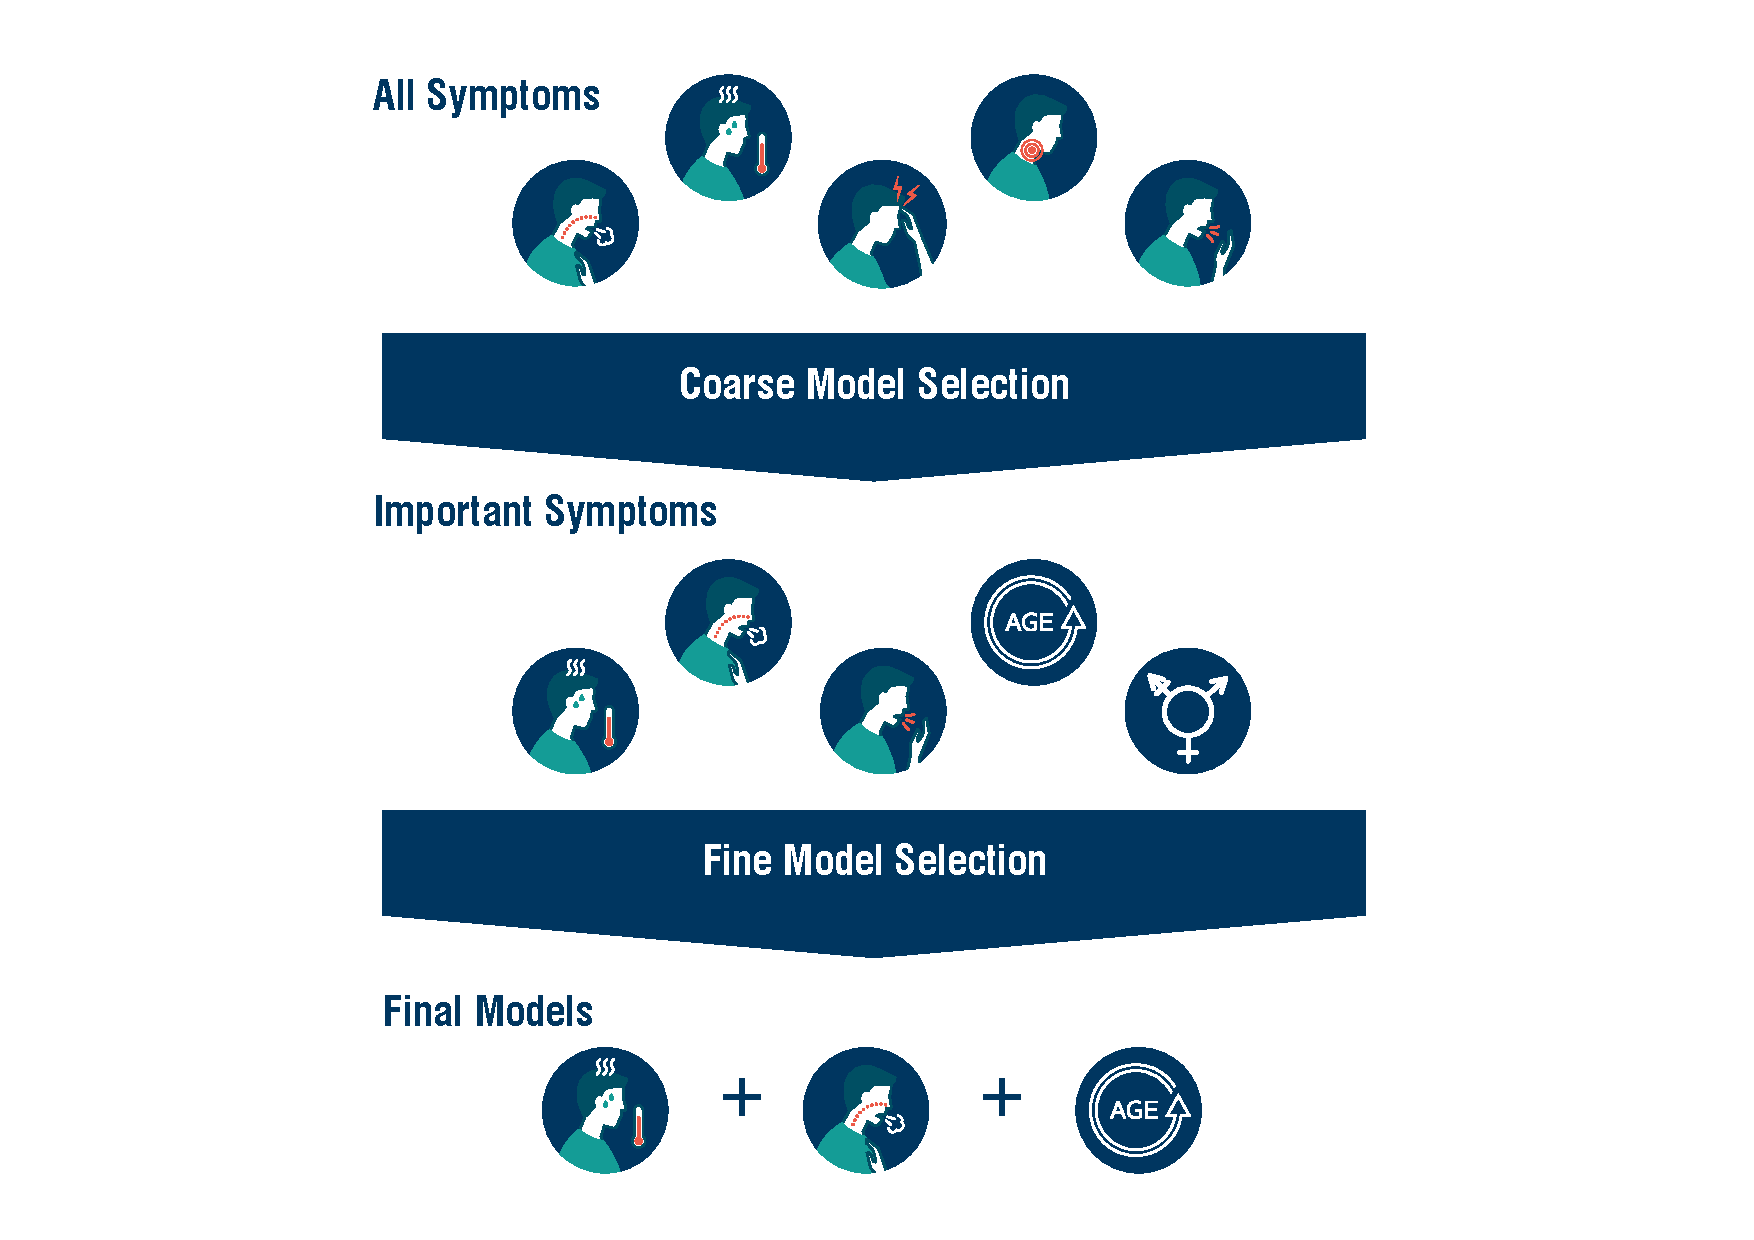
\includegraphics[width=1\linewidth]{/home/fergus/Git/COVID19_SyndromicRATDiagnosis/0500_Manuscript/0501_MainText/MainTextFigs/ModelSelectionFlowchart} \caption{Schematic for rounds of model selection in the multivariate probit component of Model Classes 2 and 3. With 14 symptoms (only 5 shown here for demonstration purposes) and two covariates there are over 131000 possible model combinations. To make exploring these possible models computationally feasible and, to reduce the risk of overfitting, we carried out two rounds of model selection. First, the data are divided into temporal cross validation sets. The multivariate probit connects symptoms to the RT-PCR result through a correlation matrix. In the coarse model selection, the most complex feasible model (all symptoms and covariates) is fit to the training data. The estimated correlations between each symptom and the RT-PCR result are compared for each cross validation set. The symptoms that have non-zero correlations in a systematic direction (i.e. all positively or all negatively correlated with RT-PCR result) are retained. The process is then repeated on each retained set of symptoms until the four symptoms in each model class with the strongest correlation to RT-PCR result. We then conduct a more exhaustive fine model selection on all the possible permutations of the four symptoms and two covariates. In this round, each model is fit to training data and used to predict for the test set, and the quality of those predictions is measured using cross entropy scoring. The cross entropy score is then used to select the best predictive model for each level of model complexity. Only these final models are then used for classification. This reduces the set of models tested as classifiers from >131 000 to just four per model class.}\label{fig:modsel-flowchart}
\end{figure}

We then compared models as classifiers using their false positive and false negative rates in three epidemiological scenarios.
In applied settings, models must often be evaluated on their performance as classifiers rather than just as prediction engines (i.e.~their ability to say a patient is COVID-19 positive or negative, not simply the probability the patient might be COVID-19 positive or negative).
To generate a classification, a probability threshold must be chosen over which patients are classified as COVID-19 positive.

Classifier performance was compared using ROC curves and error rates under three epidemiological scenarios.
ROC curves show the true and false positive rates that each model can achieve.
To extract the error rate under the epidemiological scenarios (described below), we use the ROC calculations to identify the probability threshold which most closely meets the scenario requirement (see Table \ref{tab:scenarios-tab}.
Comparing specific scenarios allows classifier performance to be demonstrated in relevant scenarios.
Whether measuring classifier performance in specific scenarios or more generally, decisions need to be made about the relative cost and acceptable levels of the two types of misclassification (false positives and negatives).
We strongly emphasise that local context should be the guide in applying these methods.

In Scenario 1, we do not consider epidemiological context but simply weight false negative and false positive rates equally by aiming to maximise the overall correct classification rate.
Scenario 2 corresponds to the current situation in Bangladesh at time of writing (July 2021), with COVID-19 cases beginning to rapidly increase again.
Under these circumstances, false negatives are extremely costly relative to false positives due to the exponential growth of the disease.
In Scenario 3, the pandemic is not declining but maintaining a steady rate of cases.
In this situation, policy-makers may be keen to keep false positive diagnoses low to prevent lockdown fatigue and to keep the workforce active.

\begin{table}

\caption{\label{tab:scenarios-tab}For each epidemiological scenario there is a requirement and a performance criterion.
The requirement refers to a base level of performance the model must achieve; in general this will be a maximum acceptable error rate of some kind.
The requirement determines a threshold for each model which most closely meets that requirement.
The performance criterion is then used to determine which model performs the 'best' given that the requirement has been met.}
\centering
\begin{tabu} to \linewidth {>{\raggedright}X>{\raggedright}X>{\raggedright}X}
\toprule
Scenario Name & Requirement & Performance Criterion (Error)\\
\midrule
1 Agnostic & Maximise correct classification rates & Sum of error rates\\
2 Rising Cases & Max. 20\% false negative rate & False negative rate\\
3 Low-Level Cases & Max. 20\% false positive rate & False positive rate\\
\bottomrule
\end{tabu}
\end{table}

\hypertarget{results-353-words}{%
\section{Results (\textasciitilde353 words)}\label{results-353-words}}

A total of 1172 subjects had data available for the current analyses.
The mean age of women participants (47\% of the sample) was 37 (SD = 14), and for men (53\% of the sample) was 36 (SD = 14).
Participants were self-selecting and drawn from across Dhaka.

Model selection for Model Class 2 (syndromic data only) and 3 (syndromic and RAT data), each retained age as an explanatory variable and showed a marked decline in predictive power at more than 4 symptoms.
The final four symptoms in order of importance (i.e.~the most important symptom was retained in all of the final 4 models, the least important symptom was only retained in the 4 symptom model) were wet cough, runny nose, loss of smell and breathing problems for Model Class 2, and fever, wet cough, tiredness and diarrhoea for Model Class 3.
For both Model Class 2 and Model Class 3 model selection retained age as a covariate but not gender.

In the comparison of model predictive performance, Model Class 1 (RAT only) performed worst with a cross entropy of 3.24 (cross entropy values further from zero correspond to worse predictive performance).
The median cross entropy values were between 2.53 and 2.59 for models in Class 2 (syndromic data only).
Models in Class 3 (combined data model) performed best with cross entropy values between 1.44 and 1.47 (see Figure \ref{fig:pred-perf}).

\begin{figure}
\centering
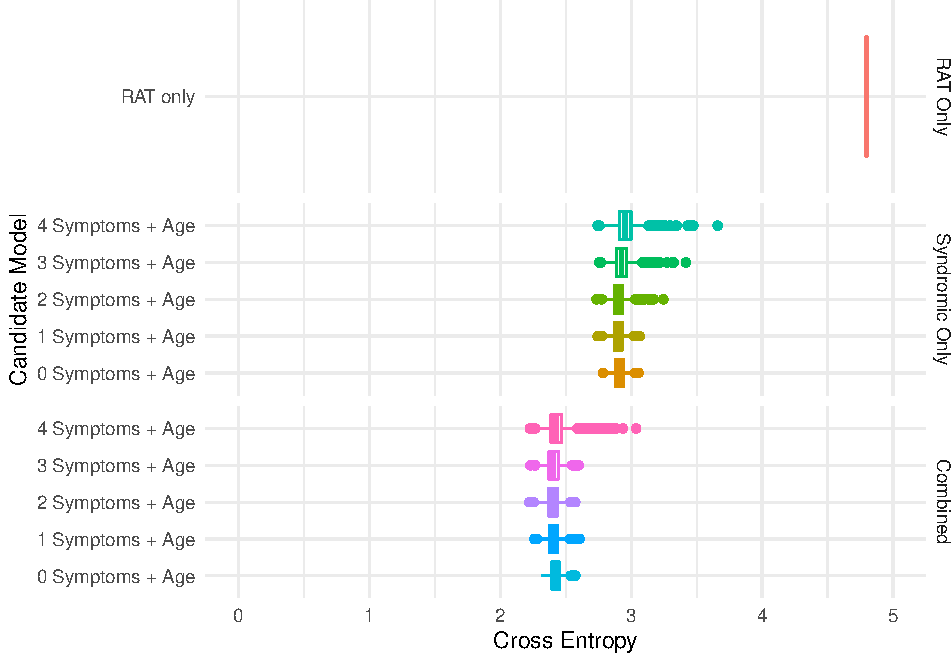
\includegraphics{0501_MainText_files/figure-latex/pred-perf-1.pdf}
\caption{\label{fig:pred-perf}Predictive performance of candidate models. Interquartile ranges for the posterior cross entropy of the best candidate models at each level of model complexity tested under temporal cross-validation. Cross entropy is a measure of distance from the truth, so values closer to zero indicate better models. The intermediate complexity models perform best at prediction, although performance is similar across all the models within each model class (1: rapid antigen testing (RAT) only; 2: syndromic data only; and 3: combined RAT and syndromic data).}
\end{figure}

General model classification performance is shown by the full ROC curves for each model (Figure \ref{fig:ROC-plot}).

Scenario specific classification performance is shown in Figure \ref{fig:scenario-plot}.
In Scenario 1 (``Agnostic,'' see Table \ref{tab:scenarios-tab}), the median error was 0.47 for models in Class 1 and Class 3 and between 0.87 and 0.9 for models in Class 2 (Figure \ref{fig:scenario-plot}).
In Scenario 2 (``Rising Cases''), Model Class 1 was unable to meet the required false negative rate.
The median errors were between
0.74 and
0.76 for models in Class 2, and
0.43 and
0.51 for models in Class 3 (Figure \ref{fig:scenario-plot}).
In Scenario 3 (``Low-Level Cases''), the error in Class 1 was 0.02 and the median errors ranged from 0.19 to 0.2 for Class 2, and 0.15 to 0.2 for Class 3 (Figure \ref{fig:scenario-plot}).

\begin{figure}
\centering
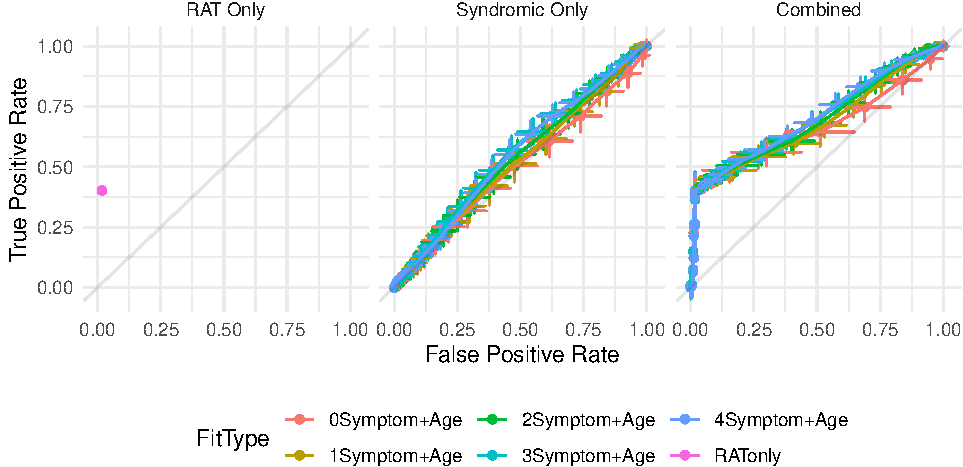
\includegraphics{0501_MainText_files/figure-latex/ROC-plot-1.pdf}
\caption{\label{fig:ROC-plot} Receiver operating characteristics for rapid antigen testing (RAT) only approach (Model Class 1) and posterior mean (+- posterior standard deviation) receiver operating characteristics for Class 2 (syndromic data only) and 3 (syndromic and RAT data) models. These curves demonstrate the performance of the model for any hypothetical scenario as defined by the axes (as opposed to Figure 5 which demonstrates model performance in specific epidemiological scenarios which are realisations of a single point in this space).}
\end{figure}

\begin{figure}
\centering
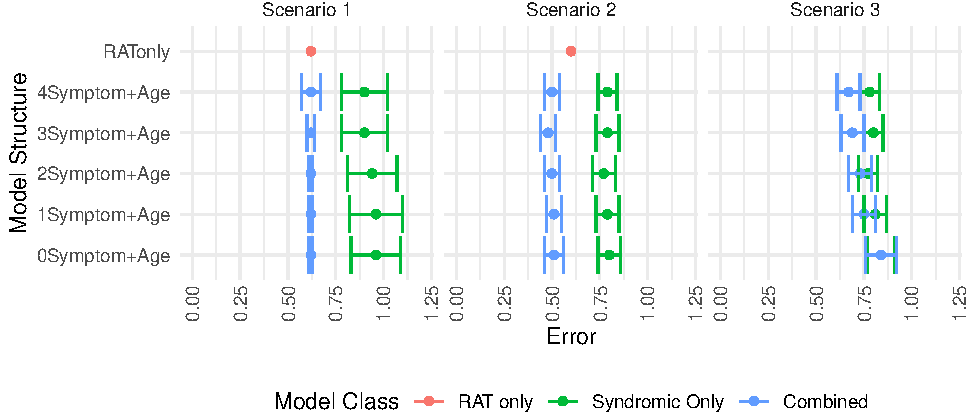
\includegraphics{0501_MainText_files/figure-latex/scenario-plot-1.pdf}
\caption{\label{fig:scenario-plot}Performance of models under each scenario measured by errors defined in Table 2. Low errors correspond to better model performance. There is no error rate defined for the Model Class 1 (RAT only model) in Scenario 2 as the model failed to meet the requirement for that scenario (making the error functionally infinite).}
\end{figure}

\hypertarget{discussion-1314-words}{%
\section{Discussion (\textasciitilde1314 Words)}\label{discussion-1314-words}}

We have demonstrated that combining rapid antigen tests (RATs) with syndromic modelling yields better prediction of COVID-19 status and greater flexibility than each diagnostic individually.
These improvements are non-trivial in real-world settings.
In Bangladesh, there are currently 15 000 new cases being identified every day, using only the limited supply of RT-PCR, the pandemic growth is accelerating and every missed case has a compounding effect.
Scenario 2 (``Rising Cases'') was developed with the need to keep false negative rates low and maps well onto the situation in Bangladesh (see Table \ref{tab:scenarios-tab}).
In this scenario, the combined data model (Model Class 3) false negative rate is
26 percentage points lower that of the RAT only model (Model Class 1).
Although the syndromic only model (Model Class 2) matches the combined models false negative rate, its false positive rate is
31 percentage points higher.
These are large performance gains for any diagnostic but when deployed at the scale of Bangladesh and similar countries, these improvements represent catching tens of thousands of cases that would otherwise be missed.
Furthermore, this boost is achieved with data that are already being collected in Bangladesh and other low- and middle- income countries (LMICs).
Outwith developing and rerunning the models presented in this paper, these improvements are essentially cost free and eminently scalable.

The pattern is similar in epidemiological Scenarios 1 (``Agnostic'') and 3 (``Low-Level Cases''), with the combined model class performing performing equally well or better than the other two classes (Figure \ref{fig:scenario-plot}).
These three scenarios only offer snapshots of performance, however, and we strongly advocate defining model performance in terms of false negative and false positive rates with reference to local conditions.
An indication of how these models will perform under any condition can be obtained by comparing the more generic model performance metrics for prediction and classification (Figures \ref{fig:pred-perf} and \ref{fig:ROC-plot}, respectively).
These figures demonstrate both the added flexibility of the more complex model classes that allow them to be tailored to specific needs and the need to combine the high-quality but inflexible RAT results with the more flexible but lower quality syndromic data.
Interestingly, the most of the Class 2 models performs approximately as well as chance except the simplest which performs worse than chance.
A model that performs worse than random can still be useful if one takes the inverse decision. \todo{@Dirk - can you please clarify this or suggest reasons the model is performing so badly. The red line here is a univariate probit regression with one continuous covariate so I don't understand why it's performing so poorly unless the temporal cross validation sets are wildly different from each other?}
Even a flexible model which performs as well as random classification can be useful if those error rates reflect those needed in a given local situation.
Fortunately, Model Class 3 is both flexible and performs better than random.

We have deliberately not emphasised the final symptoms chosen through model selection in this paper as we are focusing on prediction and classification for a unique sub-population: self-referring, symptomatic patients.
We do, however, highlight that while fever and loss of smell were the two most important symptoms in the two classes of syndromic models,
the other symptoms retained were different (with cough and wet cough retained in the combined syndromic and RAT model, Class 3, and loss of taste and vomiting in the syndromic only model, Class 2).
Further research is needed to understand the mechanisms by which symptoms predict COVID-19 and by which RAT misses COVID-19.
Of particular interest is whether individuals that are missed by RAT are less infectious, which could be explored by using Threshold Cycle (Ct) values from the RT-PCR to compare viral load with respect to prediction by the different methods {[}21{]}.
We note also that, as expected, age was retained in model selection.
We were, however, surprised that gender was removed during model selection.
Gender is thought to play a major role in infection risk {[}23{]}.
As we are looking to predict symptomatic COVID-19 in symptomatic individuals, generalised risk of infection is perhaps less predictive than expected, potentially due to the balancing of risk and burden {[}24{]}.

Using a large sample collected under field-realistic conditions, we have rigorously tested our approach.
By taking a statistical modelling approach to case identification, we are able to update our diagnostic process in real time, allowing this method to readily adapt to new variants (or even new diseases) or new priorities for resource allocation.
The modelling frameworks we have used are also sufficiently flexible to accommodate new data sources.
Of particular interest are extensions to include the ``pandemic context'' in the model using space-time data.
Furthermore, by using more sophisticated modelling structures that work at the scale of probabilities, rather than binary tests, it is possible to tune error rates to better reflect the local relative costs of false positives and false negatives.
Naturally, these strengths have complementary limitations.
Our models require updating in real-time and can only achieve good performance if the validation data are of high quality.
Similarly, targeting error rates is only sensible if those rates properly reflect local conditions which is hard to do in practice.
These limitations should be seriously considered but the alternatives for imperfect testing methods are diagnostics that cannot be tailored to local conditions at all (and, as such may perform worse than a method which is sub-optimally tailored to local conditions) or diagnostics which make these decisions implicitly and not explicitly.
We choose to make these decisions explicitly to allow them to be more readily challenged, researched and improved upon.
We also emphasise the need for rigorous experimental design to ensure findings from the sample population are applicable to the target population and the need for further research into understanding error rate trade-offs in applied settings.

We believe that the combined syndromic and rapid antigen testing approach represents the most promising approach to large-scale testing in LMICs for COVID-19 at present.
By using the small amount of RT-PCR testing possible and formally integrating multiple imperfect, non-gold-standard methods, we can tune these diagnostics to our local conditions.
We have demonstrated that these improvements can be impressive in real-world scenarios, and will have a large impact when scaled to the population sizes in LMICs.
The methodology we have outlined here is applicable to a wide range of diseases and settings across LMICs.
One of the biggest challenges in diagnosing and tracking many diseases in resource-limited settings is the low availability of access to gold-standard testing (such as RT-PCR in the case of COVID-19) and high error rates of alternative testing methods.
In this paper, we have outlined the process for coupling a small number of gold-standard tests with formal statistical integration of alternative testing methods, to generate high quality diagnostic models.
This process readily maps onto many other case identification problems, including the diagnosis of several neglected tropical diseases. For example, malaria (gold standard (GS) is also RT-PCR, imperfect methods (IM) include antigen tests, syndromic diagnosis and blood smears), schistosomiasis (GS: RT-PCR or autopsy; IM: Kato Katz egg counts, antibody detection) and rabies (GS: fluorescent antibody test; IM: light microscopy, differential diagnosis).

The management of global pandemics can only be done with global testing.
While the quest to achieve this using only gold-standard diagnostic methods is laudable, it is also often impractical.
Imperfect diagnostics are frequently imperfect in different ways, and these differences are ripe for statistical exploitation.
What is more, these approaches are often more agile than gold-standard diagnostics in situations of flux, for example, in the early stages of new pandemics or disease strains, when fast responses are essential.\\
By investing in understanding how to utilise the complementary strengths of imperfect testing and deploy the limited gold-standard testing available for validation, we can provide good quality testing at the scale needed to fight infectious diseases.

\hypertarget{funding-26-words}{%
\section{Funding (\textasciitilde26 words)}\label{funding-26-words}}

The Bill and Melinda Gates Foundation funded work by FAO (INV-022851), and University of Glasgow reports funding from Wellcome (207569/Z/17/Z).
The authors declare no competing interests.

\hypertarget{acknowledgements-67-words}{%
\section{Acknowledgements (\textasciitilde67 words)}\label{acknowledgements-67-words}}

We would like to thank members of the community support teams in Bangladesh who have provided essential services throughout the pandemic.
Earlier drafts of this mansucript benefited from the input of Daniel Haydon, Anne-Sophie Bonnet-Lebrun, Luca Nelli, Crinan Jarrett, Rita Claudia Cardoso Ribeiro, Halfan Ngowo, Heather McDevitt and Gina Bertolacci.
The University of Glasgow COVID-19 in LMICs Group provided the environment in which to develop this work.

\hypertarget{references-max-30}{%
\section*{References (Max 30)}\label{references-max-30}}
\addcontentsline{toc}{section}{References (Max 30)}

\hypertarget{refs}{}
\begin{CSLReferences}{0}{0}
\leavevmode\hypertarget{ref-corman2020detection}{}%
\CSLLeftMargin{{[}1{]} }
\CSLRightInline{Corman VM, Landt O, Kaiser M, Molenkamp R, Meijer A, Chu DK, et al. Detection of 2019 novel coronavirus (2019-nCoV) by real-time RT-PCR. Eurosurveillance 2020;25:2000045.}

\leavevmode\hypertarget{ref-tahamtan2020real}{}%
\CSLLeftMargin{{[}2{]} }
\CSLRightInline{Tahamtan A, Ardebili A. Real-time RT-PCR in COVID-19 detection: Issues affecting the results. Expert Review of Molecular Diagnostics 2020;20:453--4.}

\leavevmode\hypertarget{ref-chowdhury2020long}{}%
\CSLLeftMargin{{[}3{]} }
\CSLRightInline{Chowdhury R, Luhar S, Khan N, Choudhury SR, Matin I, Franco OH. Long-term strategies to control COVID-19 in low and middle-income countries: An options overview of community-based, non-pharmacological interventions. European Journal of Epidemiology 2020;35:743--8.}

\leavevmode\hypertarget{ref-vandenberg2021considerations}{}%
\CSLLeftMargin{{[}4{]} }
\CSLRightInline{Vandenberg O, Martiny D, Rochas O, Belkum A van, Kozlakidis Z. Considerations for diagnostic COVID-19 tests. Nature Reviews Microbiology 2021;19:171--83.}

\leavevmode\hypertarget{ref-cash2020has}{}%
\CSLLeftMargin{{[}5{]} }
\CSLRightInline{Cash R, Patel V. Has COVID-19 subverted global health? The Lancet 2020;395:1687--8.}

\leavevmode\hypertarget{ref-olalekan2020covid}{}%
\CSLLeftMargin{{[}6{]} }
\CSLRightInline{Olalekan A, Iwalokun B, Akinloye OM, Popoola O, Samuel TA, Akinloye O. COVID-19 rapid diagnostic test could contain transmission in low-and middle-income countries. African Journal of Laboratory Medicine 2020;9:1--8.}

\leavevmode\hypertarget{ref-linares2020panbio}{}%
\CSLLeftMargin{{[}7{]} }
\CSLRightInline{Linares M, Pérez-Tanoira R, Carrero A, Romanyk J, Pérez-García F, Gómez-Herruz P, et al. Panbio antigen rapid test is reliable to diagnose SARS-CoV-2 infection in the first 7 days after the onset of symptoms. Journal of Clinical Virology 2020;133:104659.}

\leavevmode\hypertarget{ref-boum2021performance}{}%
\CSLLeftMargin{{[}8{]} }
\CSLRightInline{Boum Y, Fai KN, Nikolay B, Mboringong AB, Bebell LM, Ndifon M, et al. Performance and operational feasibility of antigen and antibody rapid diagnostic tests for COVID-19 in symptomatic and asymptomatic patients in cameroon: A clinical, prospective, diagnostic accuracy study. The Lancet Infectious Diseases 2021.}

\leavevmode\hypertarget{ref-mak2020evaluation}{}%
\CSLLeftMargin{{[}9{]} }
\CSLRightInline{Mak GC, Cheng PK, Lau SS, Wong KK, Lau C, Lam ET, et al. Evaluation of rapid antigen test for detection of SARS-CoV-2 virus. Journal of Clinical Virology 2020;129:104500.}

\leavevmode\hypertarget{ref-jin2020rapid}{}%
\CSLLeftMargin{{[}10{]} }
\CSLRightInline{Jin Y-H, Cai L, Cheng Z-S, Cheng H, Deng T, Fan Y-P, et al. A rapid advice guideline for the diagnosis and treatment of 2019 novel coronavirus (2019-nCoV) infected pneumonia (standard version). Military Medical Research 2020;7:1--23.}

\leavevmode\hypertarget{ref-sim2021utilizing}{}%
\CSLLeftMargin{{[}11{]} }
\CSLRightInline{Sim JXY, Conceicao EP, Wee LE, Aung MK, Seow SYW, Teo RCY, et al. Utilizing the electronic health records to create a syndromic staff surveillance system during the COVID-19 outbreak. American Journal of Infection Control 2021;49:685--9.}

\leavevmode\hypertarget{ref-undurraga2021covid}{}%
\CSLLeftMargin{{[}12{]} }
\CSLRightInline{Undurraga EA, Chowell G, Mizumoto K. COVID-19 case fatality risk by age and gender in a high testing setting in latin america: Chile, march--august 2020. Infectious Diseases of Poverty 2021;10:1--1.}

\leavevmode\hypertarget{ref-wenham2020covid}{}%
\CSLLeftMargin{{[}13{]} }
\CSLRightInline{Wenham C, Smith J, Morgan R. COVID-19: The gendered impacts of the outbreak. The Lancet 2020;395:846--8.}

\leavevmode\hypertarget{ref-mayorga2020modelling}{}%
\CSLLeftMargin{{[}14{]} }
\CSLRightInline{Mayorga L, Samartino CG, Flores G, Masuelli S, Sánchez MV, Mayorga LS, et al. A modelling study highlights the power of detecting and isolating asymptomatic or very mildly affected individuals for COVID-19 epidemic management. BMC Public Health 2020;20:1--1.}

\leavevmode\hypertarget{ref-garry2020considerations}{}%
\CSLLeftMargin{{[}15{]} }
\CSLRightInline{Garry S, Abdelmagid N, Baxter L, Roberts N, Waroux O le P de, Ismail S, et al. Considerations for planning COVID-19 treatment services in humanitarian responses. Conflict and Health 2020;14:1--1.}

\leavevmode\hypertarget{ref-surkova2020false}{}%
\CSLLeftMargin{{[}16{]} }
\CSLRightInline{Surkova E, Nikolayevskyy V, Drobniewski F. False-positive COVID-19 results: Hidden problems and costs. The Lancet Respiratory Medicine 2020;8:1167--8.}

\leavevmode\hypertarget{ref-west2020covid}{}%
\CSLLeftMargin{{[}17{]} }
\CSLRightInline{West CP, Montori VM, Sampathkumar P. COVID-19 testing: The threat of false-negative results. Mayo clinic proceedings, vol. 95, Elsevier; 2020, p. 1127--9.}

\leavevmode\hypertarget{ref-albert1993bayesian}{}%
\CSLLeftMargin{{[}18{]} }
\CSLRightInline{Albert JH, Chib S. Bayesian analysis of binary and polychotomous response data. Journal of the American Statistical Association 1993;88:669--79.}

\leavevmode\hypertarget{ref-carpenter2017stan}{}%
\CSLLeftMargin{{[}19{]} }
\CSLRightInline{Carpenter B, Gelman A, Hoffman MD, Lee D, Goodrich B, Betancourt M, et al. Stan: A probabilistic programming language. Journal of Statistical Software 2017;76:1--32.}

\leavevmode\hypertarget{ref-gneiting2007strictly}{}%
\CSLLeftMargin{{[}20{]} }
\CSLRightInline{Gneiting T, Raftery AE. Strictly proper scoring rules, prediction, and estimation. Journal of the American Statistical Association 2007;102:359--78.}

\leavevmode\hypertarget{ref-albert2021field}{}%
\CSLLeftMargin{{[}21{]} }
\CSLRightInline{Albert E, Torres I, Bueno F, Huntley D, Molla E, Fernández-Fuentes MÁ, et al. Field evaluation of a rapid antigen test (panbio™ COVID-19 ag rapid test device) for COVID-19 diagnosis in primary healthcare centres. Clinical Microbiology and Infection 2021;27:472--e7.}

\leavevmode\hypertarget{ref-menni2020real}{}%
\CSLLeftMargin{{[}22{]} }
\CSLRightInline{Menni C, Valdes AM, Freidin MB, Sudre CH, Nguyen LH, Drew DA, et al. Real-time tracking of self-reported symptoms to predict potential COVID-19. Nature Medicine 2020;26:1037--40.}

\leavevmode\hypertarget{ref-wolff2020risk}{}%
\CSLLeftMargin{{[}23{]} }
\CSLRightInline{Wolff D, Nee S, Hickey NS, Marschollek M. Risk factors for covid-19 severity and fatality: A structured literature review. Infection 2020:1--4.}

\leavevmode\hypertarget{ref-joe2020equal}{}%
\CSLLeftMargin{{[}24{]} }
\CSLRightInline{Joe W, Kumar A, Rajpal S, Mishra U, Subramanian S. Equal risk, unequal burden? Gender differentials in COVID-19 mortality in india. Journal of Global Health Science 2020;2.}

\end{CSLReferences}


\end{document}
